\documentclass[conference, twocolumn]{IEEEtran}

\usepackage[english,french]{babel}
\usepackage{graphicx}
\usepackage{color} 
\usepackage[colorlinks]{hyperref}
\usepackage{palatino, url, multicol}
\usepackage{psfrag}
\usepackage{subfigure}
\usepackage{amsthm}
\usepackage{amsfonts}
\usepackage{amsmath}
\usepackage{algorithmic}
\usepackage{algorithm}

%\pdfpagewidth 8.5in
%\pdfpageheight 14in 

\theoremstyle{definition}

\newtheorem{definition}{Definition}[section]
\newtheorem{example}{Example}[section]

\hyphenation{op-tical net-works semi-conduc-tor}


\begin{document}

\title{On-Time Network On-Chip}

\author{Dai Bui, Alessandro Pinto \\
	Center for Hybrid and Embedded Software Systems, EECS \\
    University of California, Berkeley \\
    Berkeley, CA 94720, USA \\
    \{\tt daib, pinto\}@eecs.berkeley.edu
}

\maketitle

%\IEEEpeerreviewmaketitle
\begin{abstract}
We are moving to multi-core, however, the more cores we have, the more
communication unpredictability. Can we use multi-core in real-time embedded
systems? How do we know for sure that one packet sent from a node will reach
the destination node within a certain amount of time? We should move from
faster is better to not fast enough is wrong. In multi-core age, communication
is expensive, computation is free. For most of algorithms, running on 8 cores
will have a speed up of 1.5 due to communication overhead. We need an explicit
communication mechanism between cores running critical task. This mechanism
needs to be simple yet effient. We prove that we can achieve that by using scheduling
analysis and simulation in an cycle accurate platform. The result from
simulation matches quite well with our analysis. This approach can have a
significant impact on the design of future network on chip.

\end{abstract}

\section{Introduction}
As a network on chip gets larger, the communication on the network becomes 
very complicated. Congestions on that network can occur resulting in unpredictable 
delay in communications between network nodes. This non-deterministic behavior 
makes it very difficult to verify the timing semantics of a network on chip 
system, as a result, network on chip systems become unsuitable for real-time 
applications, especially critical control applications.

\begin{figure}[htp]
\centering
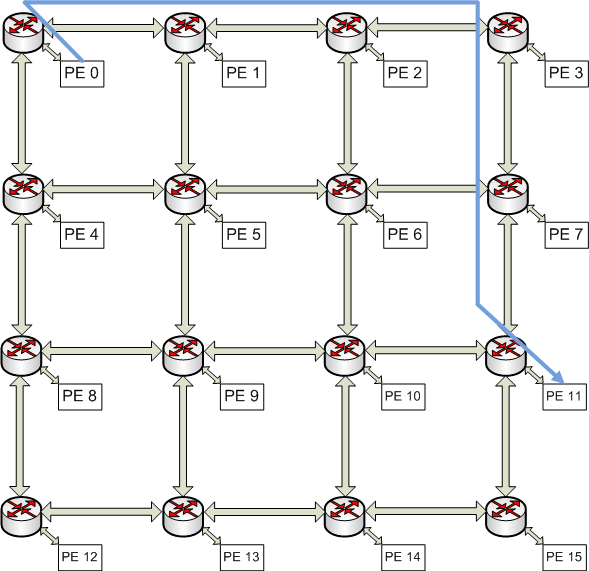
\includegraphics[width=7cm]{pics/NoC0}
\caption[Demand for a hard real-time flow.]
{How can a sending node make sure about the bounded delay for
a packet?}\label{fig:NoCRt}
\end{figure}

Our purpose is to bring the real-time communication to network on chip so that 
users can always guarantee deterministic behaviors of a critical system. To do 
so, it requires bounded delay communications between nodes in the network. 
For example, when processing element $0$ wants to send a critical control packet 
p to processing element $11$, how can it know for sure that the packet will
reach the destination within a certain amount of time? 

\section{Related Work}
\subsection{\AE thereal}
This work \cite{Goossens_chapter4} is from NXP. This architecture tries to avoid
contention using contention-free routing by {\em delaying} some packets. 

Guaranteed packets are multiplexed using TDMA. However, this approach requires
design-time configuration and verification, which is not flexible for architectures
like multi-core.
\subsection{SoCBUS}
SoCBUS architecture \cite{SoCBUS} is from Linkoping University. It seeks to 
guarantee real-time properties by setting up a path before ending:
\begin{itemize}
\item Initiate a path by sending a setting up packet.
\item The path will be {\em blocked} until all data have been sent.
\item After that the path is unlocked
\end{itemize}
This approach has the following problems: 
\begin{itemize}
\item What happens if we have two real-time paths on the same link?
\item Other traffic sharing a link with this real-time path is blocked while 
data is sent. This seems to be a good solution when sending a large bulk of data 
but not good for periodic, non-continuous flows.
\item Utilization of this approach can be low if real-time flows only require
low bandwidth.
\end{itemize}
\subsection{QNoC}
This work is from Technion \cite{QNoC}. Packets are sent synchronously. 
This architecture supports multi service levels as in table \ref{table:QNoCTable}.

\begin{table}[htbp]
\begin{center}
  \begin{tabular}{ | p{2.3cm} | p{4cm} | p{1.2cm} |}
    \hline
	Service-Level & Description & Priority \\ \hline
	Signaling & Urgent Messages, Short Packets, Interrupts, Control signals 
	requiring low transport latency & Highest \\ \hline
	Real-Time & Real-time and streaming packets & \\ \hline
	RD/WR & Short memory and register access & \\ \hline
	Block Transfer & Long messages and blocks of data & Lowest \\
    \hline
  \end{tabular}
\end{center}
\caption{QNoC Service Levels}
\label{table:QNoCTable}
\end{table}

This seems to be a good approach for soft real-time applications like video streaming
but this is not really suited for hard real-time applications since what happens 
when multiple real-time flows have to share the same link:
\begin{itemize}
\item Non-deterministic behaviors for flows.
\item Signaling packets can block real-time packets.
\end{itemize}
To solve this problem, we need to keep track of the number and specifications of
real-time flows on a link to make sure that the link is never overloaded.

\section{Our Idea}
We can achieve the real-time communication between some nodes in a network 
on a chip by borrowing the resource reservation idea \cite{Zhang93rsvp} from the 
Internet to the network on chip. In that, all the real-time communications 
have to be previously reserved on the network. 

Real-time flows can be multiplexed \cite{Ferrari90ascheme}, \cite{ZhangService}
on links in networks without violating real-time requirements. Other best-effort
flows can still use remaining bandwidth on reserved links.

An admission control mechanism is implemented, thus when a reservation 
for a real-time flow is initiated by a sender in a network, the network will determine if 
it can accept that reservation or not based on its current state of other 
reservations of other real-time flows on the network.

\begin{figure}[htbp]
\centering
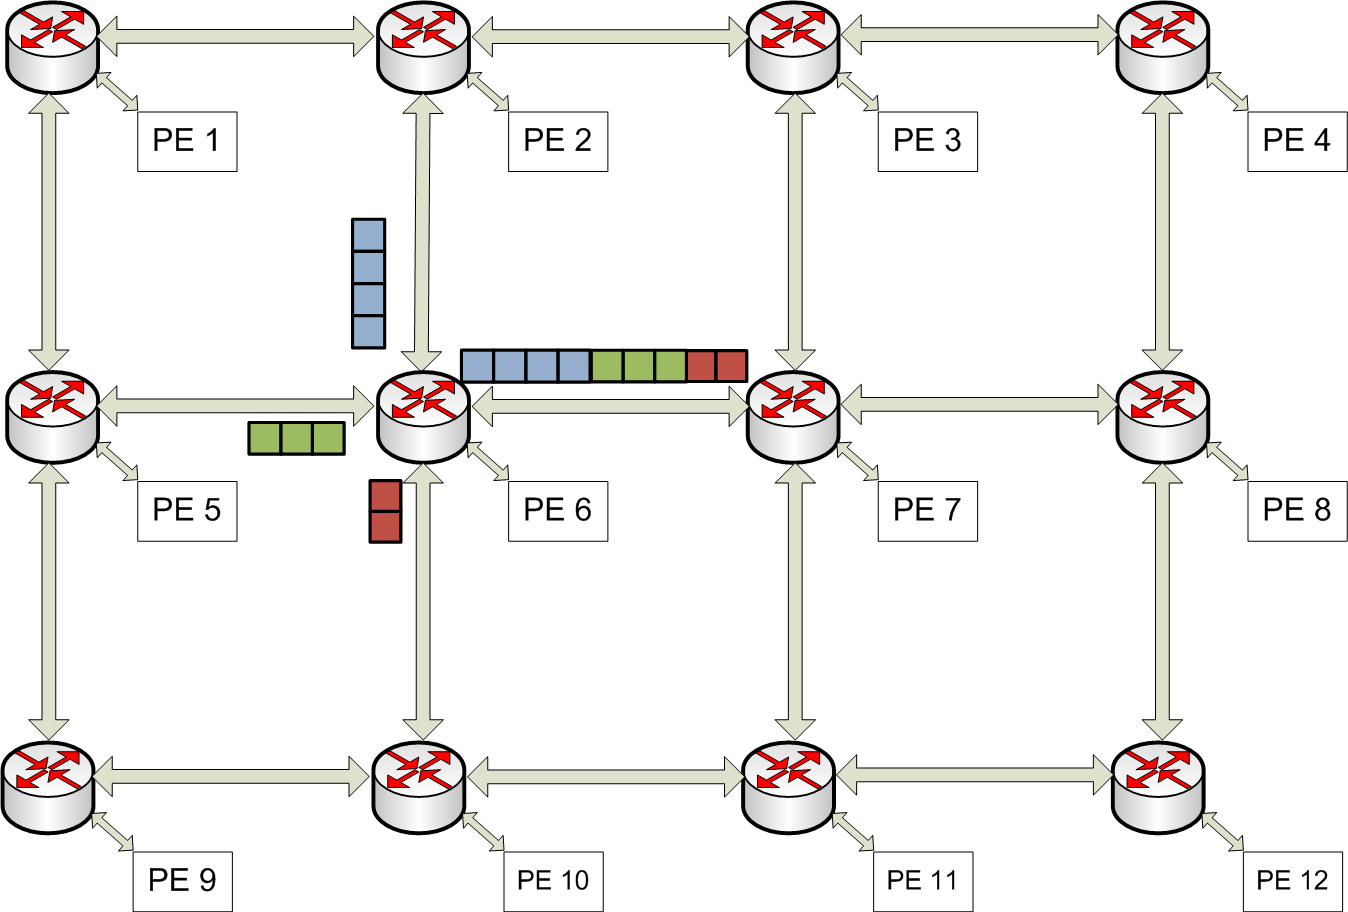
\includegraphics[width=7cm]{pics/Multiplex2}
\caption[Real time flow multiplexing.]
{Real-time flow multiplexing.}\label{fig:FlowMultiplex}
\end{figure}

\subsection{Design Goal}
\begin{itemize}
\item Multiple real-time flows can be multiplexed on one link
\cite{Ferrari90ascheme} as in Figure \ref{fig:FlowMultiplex}.
\item Utilize the spatial data paths between sources and nodes to avoid the 
conflicts between real-time flows.
\item Does not block links completely as SoCBUS \cite{SoCBUS}, best-effort flows 
still can travel links used by real-time flows.
\item Avoid unpredicted behaviors networks as in QNoC \cite{QNoC}, when there are 
multiple real-time flows suddenly travelling on the same link and their total bandwidth 
exceeds the bandwidth of the link. The admission control in our architecture can 
prevent that. Senders should always know if their required specifications for 
their communications can be met or not. 
\item Provide a reconfigurable state for real-time flows on a network, we do not 
need to pre-calculate that at {\em design time} as in \AE thereal
\cite{Goossens_chapter4}, which is really not suitable for the multi-core architecture.
\end{itemize}
\section{Formal Definitions}
\begin{itemize}
\item $t_f$ is the {\em minimum} packet interval time in cycles between two
successive packets of a real-time flow $f$.
\item $l_f$ is the {\em maximum} length of a packet in flits of real-time flow
$f$.
\item $s_{f,e}$ is the service time for a packet in a node including header 
processing, transmission time, and any other operations. $s$ is often a 
function of $l$: $s=f(l)$. We can set $s=value(l)$, this means that it takes $1$
cycle for a router to process and send one flit over a link. In pipeline router
model as in \cite{PehDelayModel}, \cite{PehSpecPipeR}, we have to add some
pipeline stages to $l$ to have $s$.
\item $T \subseteq \mathbf{N}$ is the set of the minimum interval values between
packets of flows.
\item $L \subseteq \mathbf{N}$ is the set of packet lengths.
\item $D \subseteq \mathbf{N}$ is the set of packet delays of real-time flows.
\item $\mathcal{V} \subseteq \mathbf{N}$ is the set of virtual channels between pairs of nodes.
\item $C$ is the set of {\em cores} on the on-chip network.
\item $R$ is the set of {\em routers}.
\end{itemize}

Then the set of {\em nodes} on the network is defined as:
\begin{equation}\label{reio}
V = C \cup R
\end{equation}
And $E$ defined as:
\begin{equation}
E \subseteq V \times V 
\end{equation}
is the set of {\em directed edges} between nodes in the network.

The set of {\em flows} on the network is defined as:
\begin{equation}
F \subseteq C \times C \times \mathcal{V} 
\end{equation}

And $P$ is a {\em mapping } between a real-time flows with its specifications:
\begin{equation}
P:F \rightarrow \tau \times T \times L \times D
\end{equation}
in which $\tau$ is the set of packet types.

\begin{equation}
y_{f,e} = \left\{ \begin{array}{lrc}
1 \mbox{ if flow } f \in F \mbox{ uses link } e \in E \\
0 \mbox{ otherwise} 
\end{array}\right.
\end{equation}

\begin{equation}
\delta_{f,v} = \left\{ \begin{array}{lrc}
1 \mbox{ if flow } f \in F \mbox{ going through node } v \in V \\
0 \mbox{ otherwise} 
\end{array}\right.
\end{equation}

\begin{equation}
\sigmal_{f,e} = \left\{ \begin{array}{lrc}
1 \mbox{ if flow } f \in F \mbox{ has the largest maximum packet length of all
flows on } e \in V \\ 
0 \mbox{ otherwise} 
\end{array}\right.
\end{equation}

\begin{equation}
I_{v,e} = \left\{ \begin{array}{lrc}
1 \mbox{ if } e \in E \mbox{ is outgoing edge from } v \in V \\
-1 \mbox{ if } e \in E \mbox{ is incoming edge from } v \in V \\
0 \mbox{ otherwise}
\end{array}\right. 
\end{equation}

$\forall f=(s, d, id) \in F$  let $b$ be a vector s.t. $b_f(s) = 1$, 
$b_f(d) = -1$ and $b_f(i) = 0, \forall i \in C \mbox{ and } i \neq s, d$,
 then we have $Iy_f=b_f$, this condition is for unique path between $s$ and $d$.

Configuration $\mathcal{C}(F)=(P, \{y_f\}_{f \in F})$.
\section{Architecture}
At each node in a router, we employ the Internet stack to each node in the 
network on chip.
\begin{table}[h]
\begin{center}
  \begin{tabular}{ | l | }
    \hline
    Application layer at processing units \\ \hline
    Transport layer at processing units \\ \hline
    Network layer at routers \\ \hline
	Data link layer at routers \\ \hline
	Physical layer \\
    \hline
  \end{tabular}
\end{center}
\caption{Network stack model}
\label{table:NetworkStack}
\end{table}

\subsection{Path Setup Protocol}
When in need of a real-time communication, the processing unit at each node 
will issue a request for setting up a path:

{\em Setuppath.request(source\_id, destination\_id, virtual\_channel\_id T, L,
D);}

\begin{figure}[htp]
\centering
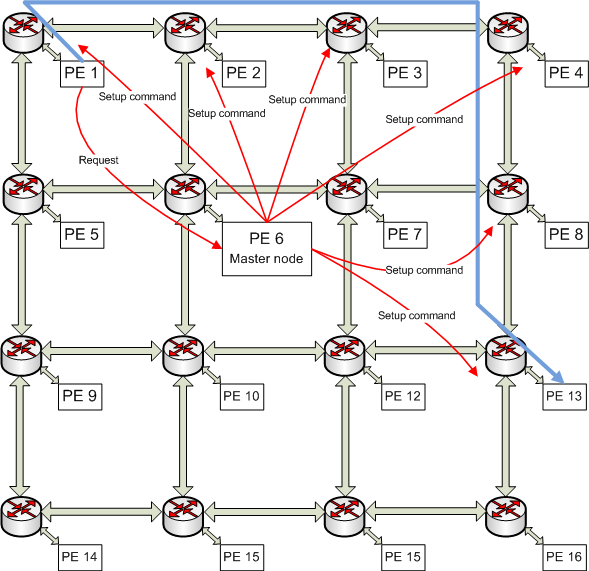
\includegraphics[width=7cm]{pics/Protocol2}
\caption[Setup request for a real-time flow.]
{Real-time flow setup protocol.}\label{fig:ReqSetup}
\end{figure}

This request will be sent over the network by a REQ message to a specific node
in the network, called {\em master node}, as in Figure \ref{fig:ReqSetup}.
Based on its knowledge about other flows in the network and the demand for the
new real-time flow, the master node will seek to find a suitable path. If there
exists a suitable path, the master node will send SETUP command messages to
appropriate routers in the network to configure routers' configurations. This
re-configuration can include adjusting configurations of other flows at the routers.

Routers receiving SETUP command message will adjust their internal
configurations as specified in the message. After finishing setting up internal
configurations, routers will send back an acknowledgement ACK message to
the master node. When the master node have received all its expected ACK
messages from routers, it sends an ACCEPT message to the requesting node
(node requested a new real-time flow). The requesting node can start sending
data after receiving that ACCEPT message.

If the master node cannot find a suitable path, it sends back to the requesting
node a REJECT message saying that new real-time flow cannot be set up on the
network.

So the setting up path response can be: ACCEPT, REJECT

When a path is not needed, it can be torn using path-tearup protocol, which
works basically as the path-setup protocol but with reversed commands.

\subsection{Design Questions}
\begin{itemize}
\item Should we specify the path directly in this request? Static initialization 
can be useful in some programming model like Giotto.	
\item Is it possible that the acceptance message will be blocked on the network 
or it reaches the source too late? We should give priority to such kind of control
message.
\item Real-time flows block other best-effort packets traveling on the link when 
the utilization of all the packets on the link is $1$. We need a mechanism to
reroute all best-effort packets.
\end{itemize}

To reduce the size of each router, we can use processing elements to do 
complicated tasks like calculating admission criteria for a new flow at each node 
and rerouting for finding a new suitable path on a network.


One interesting characteristic of this scheme is that the buffer for each 
real-time flow at each node is bounded \cite{Ferrari90ascheme}, and thus
real-time packets can be sent {\em asynchronously} resulting in better bandwidth
since we do not have to send {\em acknowledgement} for each flit sent. So at
data link layer, we employ heterogeneity communications, {\em synchronous}
communications for best effort packets and {\em asynchronous} communications
for real-time packets as in Figure \ref{fig:HeteroComm}. Best-effort packets
are preemptible by real-time packets. Real-time packets are not preemptible.
Since real-time flits does not need acknowledgement so the speed of sending
real-time packets is two time faster than best-effort packets.


\begin{figure}[htbp]
\centering
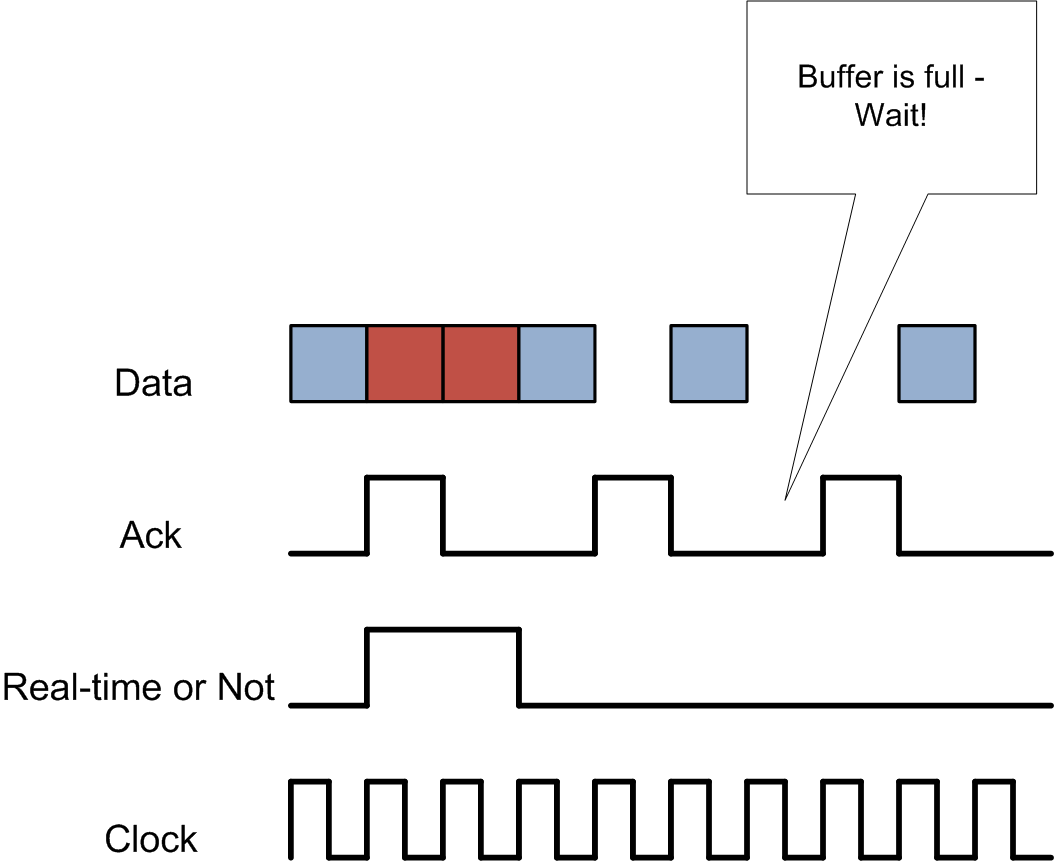
\includegraphics[width=8cm]{pics/HeteroComm.png}
\caption[Heterogeneous Communication for Packets.]
{Real-time packets and best-effort packets are treated
differently.}\label{fig:HeteroComm}
\end{figure}

\section{Theoretical Foundations}
\subsection{Delay Model in Cut-through Networks}

The delay model in \cite{Ferrari90ascheme}, \cite{VermaJitter91} is
for store-forward networks \cite{DallyPrinNetwork} (a packet has to be
received {\em completely} by a router before it can be forwarded). However, we
are considering cut-through networks (a packet can be sent while being
received) since it has better throughput.

{\textbf{Definitions:}}
$q_{f,v}$ is the {\em maximum} delay of a {\em flit} in flow $f$ at
hop (router) $v$ in cycles.This is the {\em queueing} delay.

The delay at each node of a packet is defined as the duration from the header
of that  packet is received until the header is started to send, then we do not
need to include the service time of the packet itself at the node. The {\em
minimum} local delay of a packet at a node is thus the same as the maximum
delay of a flit at a node since we do not allow preempting real-time packets. In
\cite{Ferrari90ascheme}, the delay is :

\begin{equation}\label{equ:nodedelay1}
q_{i,n} = \sum_{j=1}^{i-1}s_{j,n}+s_{max} \forall i = 1, ..., K
\end{equation}

 
$p_{f,e}$ is the propagation delay of a {\em flit} of flow f on link $e
\in E$. In network on chip, $p_e=1 \forall e \in E$.

$r_{v,f,u}$ is the time of flit $u$ of flow $f$ reach node $v$.  

$d_{f,e}$ is the {\em maximum} delay of flow $f$ on link $e$ measured in
cycles. This delay is the period between the time a flit reaches one node:
\begin{equation}\label{equ:edgeDelay}
d_{f,e} = q_{f,v}\delta_{f,v} + p_{e} = q_{f,v}\delta_{f,v} + 1 
\end{equation}

and
\begin{equation} 
d_{f,e}y_{f,e} \geq I_{v,e}y_{f,e}r_{v,f,e} + I_{v',e}y_{f,e}r_{v',f,e}
\end{equation}

From \cite{Ferrari90ascheme}, for simplicity, if we assume that all $K$ 
real-time flows going through a node $n$ satisfy the following condition:
\begin{equation}\label{equ:intervalservice1}
t_i \geq \sum_{j=1}^Ks_{j,n}, \forall i = 1,...,K
\end{equation}
the inequality (\ref{equ:intervalservice1}) can be expressed in the flowing way:
\begin{equation}
t_f y_{f,e}\geq \sum_{f^{'} \in F} s_{f^{'}}y_{f^{'},e}, \forall e \in E
\end{equation}
or
\begin{equation}\label{equ:intervalservice3}
P(f)(2) y_{f,e}\geq \sum_{f^{'} \in F} s_{f^{'}}y_{f^{'},e}, \forall e \in E
\end{equation}
This means that no deadlines for subsequent packets of a real-time flow will
fall within the interval between time $t_0$ and $t_0 + \sum s = t_0 +
\sum_{j=1}^Ks_{j,n}$.

We define a function $order_{v,e}(f)$ over the set of all real-time flows $F$
as a function to determine if there are two packets $p_1$ and $p_2$, arriving at
a node $v$ at the same time of two real-time flows $f1$ and $f2$ respectively
and competing for an output link $e$, packet $p_1$ will be sent before $p_2$ if
$order_{v,e}(f_1) < order_{v,e}(f_2)$. 

\begin{figure}[htbp]
\centering
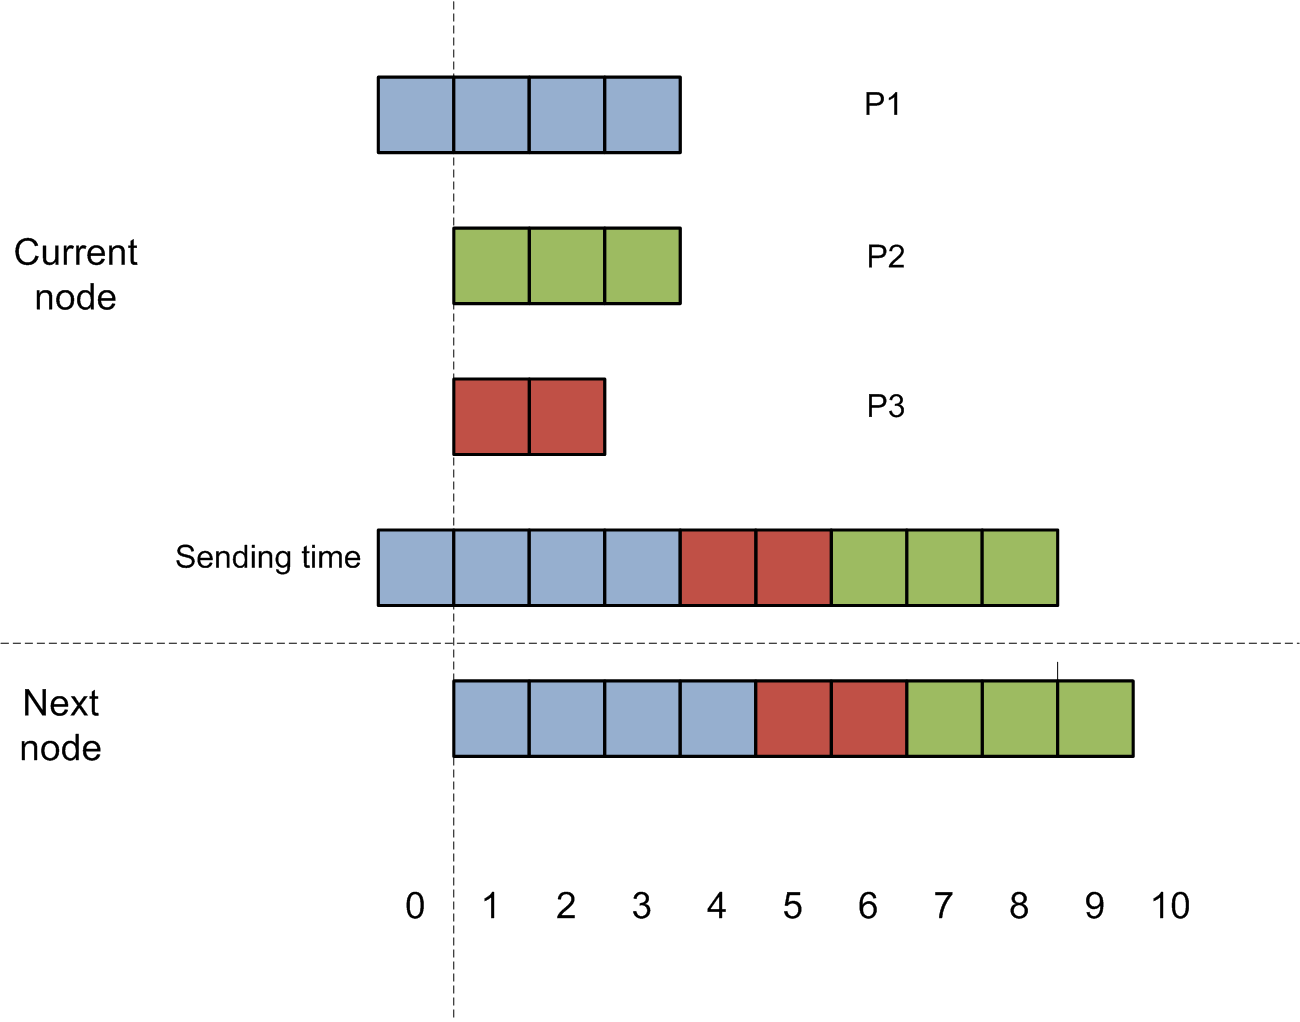
\includegraphics[width=8cm]{pics/DelayModel.png}
\caption[Delays for packets.]
{Delay Model.}\label{fig:DelayModel}
\end{figure}

In our cut-through network, the local delay at each node is a little bit
different from \cite{Ferrari90ascheme} as shown in the below equation:

\begin{eqnarray}\label{equ:queueDelay}
q_{f,v}y_{f,e} = \sum_{g \in F:order_v(g) <
order_v(f)}\delta_{g,v}y_{g,e}s_{g,e} + \notag \\ 
max(s_{i \in F}y_{i,e})-1, \forall e \in E
\end{eqnarray}

The detail analysis of (\ref{equ:queueDelay}) is that: From Figure
\ref{fig:DelayModel}, if we suppose $p_i$ is a packet of flow $f_i$, and
$order_{v,e}(f_1) < order_{v,e}(f_2) < order(f_3)$, then we can easily see that
the bounded {\em queueing} delay for packets $p_1$ and $p_2$ are 3 and 5
respectively as computed by quation (\ref{equ:queueDelay}). However, the bounded
queueing delay for packet $p_3$ is 5 if it comes at the the same time as $p_1$ and $p_2$. So we
have the bounded delay for a packet of a real-time flow that has {\em largest
maximum} packet length is:

\begin{eqnarray}\label{equ:queueDelayMaxPacketFlow}
q_{f,v}y_{f,e} = \sum_{g \in F:order_v(g) <
order_v(f)}\delta_{g,v}y_{f,e}s_{f,e}
\end{eqnarray}

The local (queueing) delay (\ref{equ:queueDelay}) has to be subtracted one since
the notion of time in \cite{Ferrari90ascheme} is continuous so that time $0+$ is basically $0$ but in
our network with the notion of time is discrete, the time $0+$ is $1$ cycle
latter.

From (\ref{equ:edgeDelay}) and
(\ref{equ:queueDelay})(\ref{equ:queueDelayMaxPacketFlow}) we then have:

\begin{eqnarray}\label{equ:edgeDelay2}
d_{f,e}y_{f,e} = \sum_{g \in F:order_v(g) < order_v(f)}y_{f,e}s_{f,e} + \notag
\\ max(s_{i \in F}y_{i,e}), \forall e \in E
\end{eqnarray}

If $f$ is the flow that has largest maximum packet length:

\begin{eqnarray}\label{equ:edgeDelayMaxPacketFlow1}
d_{f,v}y_{f,e} = \sum_{g \in F:order_v(g) <
order_v(f)}\delta_{g,v}y_{f,e}s_{f,e} + 1
\end{eqnarray}

If we set $order_{v,e}(f)=l_f$, the maximum packet length of flow $f$, then
(\ref{equ:edgeDelay2}) becomes:

\begin{eqnarray}\label{equ:edgeDelayPacketLength}
d_{f,e}y_{f,e}(1-\sigma_{f,e}) = \left(\sum_{g \in F:l_g <
l_f}y_{g,e}s_{g,e} + max(s_{i \in F}y_{i,e})\right) \notag \\
(1-\sigma_{f,e}), \forall e \in E
\end{eqnarray}

and (\ref{equ:edgeDelayMaxPacketFlow1}) becomes:

\begin{eqnarray}\label{equ:edgeDelayMaxPacketFlow2}
d_{f,v}y_{f,e}\sigma_{f,e} = \left(\sum_{g \in F:l_g <
l_f}\delta_{g,v}y_{g,e}s_{g,e} + 1\right)\sigma_{f,e}, \forall e \in E
\end{eqnarray}

This means that flows with smaller maximum packet lengths will be given smaller
delays at this node (thereby smaller deadlines when packets come at the same
time). This ordering scheme will give the smallest {\em overall} delay at this node.

However, from (\ref{equ:edgeDelayPacketLength})
and (\ref{equ:edgeDelayMaxPacketFlow2}), can see that there is a case that, at
a node, the bounded delay of flow $f$ with largest packet length will be {\em
smaller} than the bounded delay of some other flow with smaller maximum packet
length. To still use (\ref{equ:deadline1}), we have to assign a {\em virtual
delay} for the flow $f$ so that this {\em virtual deadline}, computed from
(\ref{equ:deadline1}), is greater than the any other delay of other flows to
make sure that, if all the packets of all flows comes at the same time, the packet
of the flow $f$. We will prove that, this virtual delay scheme for the flow
{\em does not} make any packet of the flow miss its deadline and the delay
bound of a packet is still the same as in (\ref{equ:edgeDelayMaxPacketFlow1}).
This virtual delay is set to the largest bounded delay of all other flows
sharing the same link.

{\textbf{Theorem 1:}} {\em  The above virtual dealy scheme never makes
packets of flow $f$ miss their real deadlines computed from
(\ref{equ:deadline1}) and (\ref{equ:edgeDelayMaxPacketFlow1})}.

{\em Prove:} Suppose that $\mathcal{S}$ is the total maximum service time of all
other flows except $f$. So the real delay bound of $f$ is $\mathcal{S}+$1.
Suppose that a packet $p$ of $f$ comes at time $t_0$, then the {\em real}
deadline for the packet is $t_0+\mathcal{S}+$1. Since from
(\ref{equ:intervalservice3}), we now that each flow can not have more than 1
packet between the duration ($t_0, t_0+\mathcal{S}+$1). If between $t_0,
t_0+\mathcal{S} -$1, there is an any cycle that no flit of other packets is
sent, then the scheduler will immediately start forwarding packet $p$ of flow $f$.
Otherwise, at time $t_0+\mathcal{S}$, all the flits of other packets are
forwarded, then the packet $p$ is started forwarding and its header will reach
the next node at $t_0+\mathcal{S}+$1. The real delay bound is satisfied.

\subsection{Configuration}
A valid configuration $\mathcal{C}(F)$ must satisfy (\ref{connectivity1}) 
(\ref{equ:e2eDelayST}) (\ref{equ:intervalservice3}) (\ref{equ:utilization1})

\begin{equation}\label{connectivity1} Iy_f=b_f,\forall f \in F
\end{equation}

The total delay at each hop of a real-time flow has to satisfy the delay constraint
of the real-time flow.

\begin{equation}\label{equ:e2eDelayST}
\sum_{e \in E}d_{f,e}y_{f,e} \leq P(f)(4), \forall f \in F
\end{equation}

When multiple real-time flows share the same link, the following conditions
 have to be met on each shared link \cite{Ferrari90ascheme},
 \cite{VermaJitter91}:

\begin{equation}\label{equ:utilization1}
\sum_{f \in F}\frac{s_{f,e}}{P(f)(2)}y_{f,e} \leq 1, \forall e \in E
\end{equation}

Since $S$ is a function of the packet length, for a simple (non-pipeline) router
model, we often have $s=P(f)(3)$, then (\ref{equ:utilization1}) becomes:

\begin{equation}\label{equ:utilization2}
\sum_{f \in F}\frac{P(f)(3)}{P(f)(2)}y_{f,e} \leq 1, \forall e \in E
\end{equation}

At each node, we use Earliest Deadline First (EDF) \cite{VermaJitter91} 
to schedule packets, the deadline for each packet of flow $f$ at node $n^{th}$
is computed as follows: 
\begin{equation}\label{equ:deadline1}
dl_{f,n}=t_0 + \sum_{k=1}^{n}q_{f,k}+P_n
\end{equation}
where $t_0$ is the time the packet is sent from the source and $P_n$ is the propagation
delay from the source till node $n^{th}$ (communication time). We set
$P_n=n$ since in network on chip, it takes one cycle for a head flit to travel
between two successive nodes. Thus, (\ref{equ:deadline1}) becomes:

\begin{equation}\label{equ:deadline2}
dl_{f,n}=t_0 + \sum_{k=1}^{n}d_{i,k}
\end{equation}

However (\ref{equ:e2eDelayST}) is for a store-forward networks, in a
cut-through network, it becomes
\begin{equation}\label{equ:e2eDelayCT}
\sum_{e \in E}d_{f,e}y_{f,e} + (s_f - 1) \leq P(f)(4), \forall f \in F
\end{equation}
since we have to include the service time, $s_f-1$, for a packet of flow $f$ at
the last node to receive {\em remaining} flits in the packet, not only the
header.

For simple router models (non-pipeline), we have $s_f = P(f)(3)$, then
(\ref{equ:e2eDelayCT}) becomes:
\begin{equation}\label{equ:e2eDelayCTNonPipeline}
\sum_{e \in E}d_{f,e}y_{f,e} + P(f)(3) - 1 \leq P(f)(4), \forall f \in F
\end{equation}

From (\ref{equ:edgeDelayPacketLength})(\ref{equ:edgeDelayMaxPacketFlow2})and
(\ref{equ:e2eDelayCTNonPipeline}) we have:
\begin{eqnarray}\label{equ:e2eDelayCTNonPipeline1}
\sum_{e \in E} \Biggl((\sum_{\forall g \in F:l_g <
l_{f}}y_{g,e}s_{g,e}+max(s_{i \in F}.y_{i,e}))(1-\sigma_{f,e}) +
\notag \\ 
\sigma_{f,e}(\sum_{g \in F:l_g <
l_f}\delta_{g,v}y_{g,e}s_{g,e} + 1)\Biggr) y_{f,e} \notag \\ \leq
P(f)(4)-P(f)(3) + 1, \forall f \in F
\end{eqnarray}

Now a valid configuration $\mathcal{C}(F)$ has to satisfy (\ref{connectivity1}) 
(\ref{equ:utilization2})
(\ref{equ:intervalservice3}) (\ref{equ:e2eDelayCTNonPipeline1})

\subsection{Dynamic Path Establishment and Routing}
When a new real-time path needs to be set up with some specifications, we have:
$F \rightarrow F \cup \{f^{'} \}=F^{'}$
and $T \rightarrow T^{'}$ s.t. $T^{'} (f)=T(f)\forall f \in F$ and $T^{'}
(f^{'})=(\tau ^{'}, T^{'}, L^{'}, D^{'})$.

The problem becomes: Find $y_{f^{'}e}$ s.t. $\mathcal{C}(F^{'})$ is valid
when we know that $\mathcal{C}(F)$ is valid.

For a new configuration $\mathcal{C}(F^{'})$, we find a new flow $f^{'}$ such that
the conditions (\ref{connectivity1})(\ref{equ:utilization2}) are satisfied. And
the path delay constraint from (\ref{equ:e2eDelayCTNonPipeline}) is:
\begin{eqnarray}\label{equ:e2eDelayNewPath}
\sum_{e \in E} \Biggl((\sum_{\forall g \in F:l_g <
l_{f'}}y_{g,e}s_{g,e}+max(s_{i \in F}.y_{i,e}))(1-\sigma_{f,e}) +
\notag \\ 
\sigma_{f,e}(\sum_{g \in F:l_g <
l_f'}\delta_{g,v}y_{g,e}s_{g,e} + 1)\Biggr) y_{f',e} \notag \\ \leq
P(f')(4)-P(f')(3) + 1,  f' \in F
\end{eqnarray}

If we assume the maximum service time for one packet on an edge of a flow is the
same for all edges (which is true for network on chip) and again the router
model is simple (non-pipeline) then we have:
\begin{eqnarray}\label{equ:e2eDelayNewPath2}
\sum_{e \in E} \Biggl((\sum_{\forall g \in F:l_g <
l_{f}}y_{g,e}s_{g,e}+max(s_{i \in F}.y_{i,e}))(1-\sigma_{f,e}) +
\notag \\ 
\sigma_{f,e}(\sum_{g \in F:l_g <
l_f}\delta_{g,v}y_{g,e}s_{g,e} + 1)\Biggr) y_{f,e} \notag \\ \leq
P(f)(4)-P(f)(3) + 1,  f' \in F
\end{eqnarray}

To add a new real-time flow like this to the network without modifying the paths
of other previous real-time flows, we store a {\em slack} of delay for each
real-time flow. Then whenever we add a new real-time flow and modify the local
bounded delay of other flows we check if the increasing delay amounts of the
flows exceed the slack of the flows and then recompute new slacks for these
flows. The slack of a flow $f$ is computed as:

\begin{eqnarray}\label{equ:slack1}
	slack_f=P(f)(4)-P(f)(3) + 1 - \notag \\ 
	\sum_{e \in E} \Biggl(\sum_{\forall g \in F:l_g <
l_{f}}\left(y_{g,e}s_{g,e}+max(s_{i \in F}.y_{i,e})\right)(1-\sigma_{f,e}) +
\notag \\ 
\sigma_{f,e}(\sum_{g \in F:l_g <
l_f}\delta_{g,v}y_{g,e}s_{g,e} + 1)\Biggr) y_{f,e}, \notag \\ 
	\forall f \in F
\end{eqnarray}

With this scheme, we have to modify the configurations of other flows sharing
the same link with the new flow. The master node will issue a SETUP command to
override the previous configurations at routers.

If a new flow $f'$ is requested, then employing {\em shortest maximum packet
length first} ordering requires to modify the delay of flows at sharing some
links with $f'$ that have larger maximum packet lengths larger than the new flow
maximum packet length. 

$\forall f \in F$  that $l_{f'} < l_f$ and $y_{f',e}y_{f,e}=1 \mbox{ for some }
e \in E$, from (\ref{equ:e2eDelayCTNonPipeline1}) we have:

\begin{eqnarray}\label{equ:e2eDelayModification}
\begin{eqnarray}\label{equ:e2eDelayCTNonPipeline1}
\sum_{e \in E} \Biggl((\sum_{\forall g \in F:l_g <
l_{f}}y_{g,e}s_{g,e}+max(s_{i \in F}.y_{i,e})+y_{f',e}s_{f',e})(1-\sigma_{f,e})
+ \notag \\ 
\sigma_{f,e}(\sum_{g \in F:l_g <
l_f}\delta_{g,v}y_{g,e}s_{g,e} + 1)\Biggr) y_{f,e} \notag \\ \leq
P(f)(4)-P(f)(3) + 1, \forall f \in F
\end{eqnarray}

or

\begin{eqnarray}\label{equ:e2eDelayModificatio2}
\sum_{\forall e \in E}y_{f',e}s_{f',e} \leq P(f)(4)-P(f)(3) + 1 - \notag \\ 
	\sum_{e \in E} \Biggl(\sum_{\forall g \in F:l_g <
l_{f}}\left(y_{g,e}s_{g,e}+max(s_{i \in F}.y_{i,e})\right)(1-\sigma_{f,e}) +
\notag \\ 
\sigma_{f,e}(\sum_{g \in F:l_g <
l_f}\delta_{g,v}y_{g,e}s_{g,e} + 1)\Biggr) y_{f,e}, \notag \\ 
	\forall f \in F
\end{eqnarray}

or

\begin{equation}\label{equ:e2eDelayModificatio3}
\sum_{\forall e \in E}y_{f',e}s_{f',e} \leq slack_f, \forall f \in F
\end{equation}

\section{Specifications}
\subsection{Message Structures}

There are two type of packets in best-effort flow identified by the head flit
in a packet. The head flit can be of CTRL (control) or HEAD (normal) type. The
structure of a REQ message (this is often a flit) to set up a real-time flow on the network is:

\begin{table}[htbp]
\begin{center}\resizebox{8cm}{!}{
  \begin{tabular}{ | l | l | l | l | l | l | l | l | }
    \hline
	CTRL & Req Node ID & Master Node ID & \multicolumn{2}{|c|}{REQ} \\ \hline
	BODY & Source ID & Destination ID & \multicolumn{2}{|c|}{$t_{min}$} \\ \hline 
	TAIL & \multicolumn{2}{|c|}{Virtual Channel ID} & $l_{max}$ & $d_{max}$ \\
    \hline
  \end{tabular}
}
\end{center}
\caption{REQ path message}
\label{table:PathMsg}
\end{table}

The SETUP message from the master node to router has the following structure:

\begin{table}[htbp]
\begin{center}\resizebox{8cm}{!}{
  \begin{tabular}{ | l | l | l | l | l | l | l | l | } 
    \hline 
	CTRL & Master ID & Router ID & SETUP & Local delay \\ \hline
	TAIL & \multicolumn{2}{|c|}{Virtual Channel ID} & Input gate & Output gate 	\\
    \hline
  \end{tabular}
}
\end{center}
\caption{SETUP path message}
\label{table:PathMsg}
\end{table}

The ACK or ACCEPT message has the following form:


\begin{table}[htbp]
\begin{center}\resizebox{8cm}{!}{
  \begin{tabular}{ | l | l | l | l | l | l | l | l | }
    \hline
	CTRL & Source ID & Destination ID & (ACK or ACCEPT) \\ \hline
	TAIL & \multicolumn{2}{|c|}{Virtual Channel ID} &  \\
    \hline
  \end{tabular}
}
\end{center}
\caption{SETUP path message}
\label{table:PathMsg}
\end{table}


The structure of a real-time data packet is:

\begin{table}[htbp]
\begin{center}\resizebox{8cm}{!}{
  \begin{tabular}{ | l | l | l | l | l |}
    \hline
	HEAD & Virtual Channel ID & jitter & Data \\ \hline 
	BODY & \multicolumn{3}{|c|}{Data flit} \\ \hline
	BODY &\multicolumn{3}{|c|}{...} \\ \hline
	TAIL & \multicolumn{3}{|c|}{Data flit} \\
    \hline
  \end{tabular}
}
\end{center}
\caption{Real-time data message}
\label{table:DataMsg}
\end{table}

\subsection{Considerations}

\begin{figure}[htp]
\centering
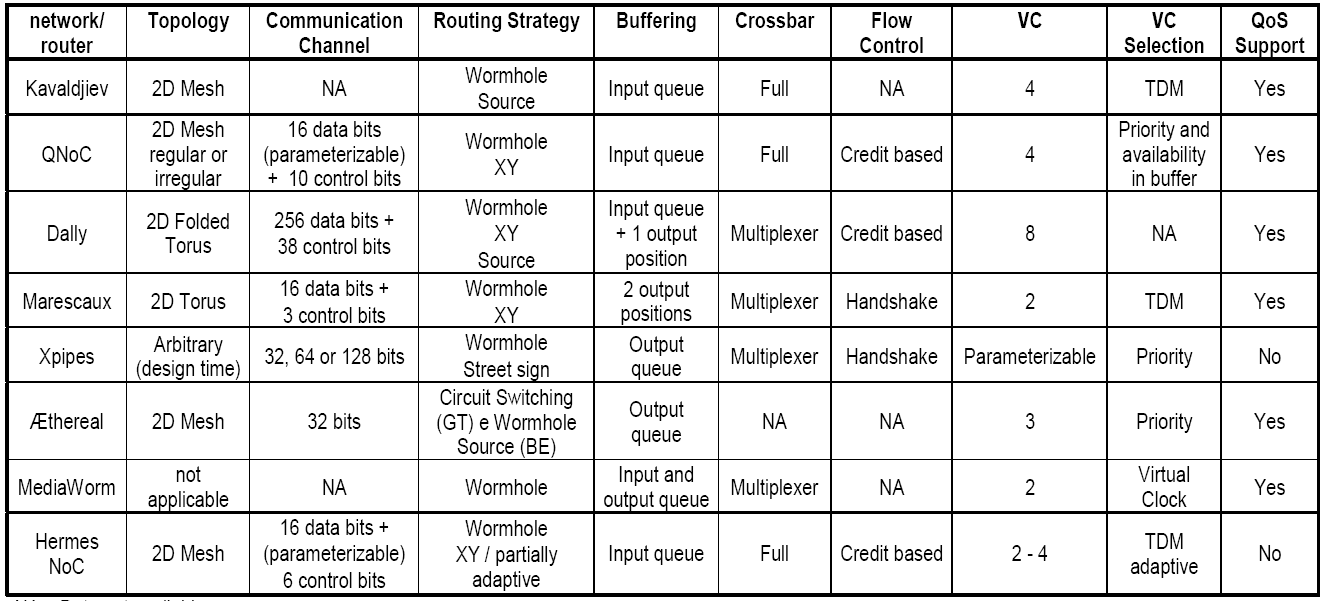
\includegraphics[width=8cm]{pics/OtherArcs.png}
\caption[Other Spec.]
{Specification of other network on chip architectures}\label{fig:otherSpec}
\end{figure}

From this we can consider the format of a data packet since we have the 
tradeoff between the length of a packet and the bounded delay of the packet. 
If the packet is long, then our network is more efficient, however, the bounded 
delay will probably large.

\subsection{Cut-Through Router Structure}

Figure \ref{fig:RouterStructure} show the structure of a router. In a router,
each input has one {\em priority} queue for real-time packets of each output.
Packets in the priority queue is {\em ordered} by deadline as in
\ref{equ:deadline2}. Each output will pick the top packets from priority queues
and compare their deadlines to find the packet with closest deadline and this
packet is selected to send. Best-effort packets are stored in FIFO queues as in
normal routers. The router is a cut-through router so that one packet can be
compared the deadline and forwarded right at the time its header each a node.

\begin{figure}[htp]
\centering
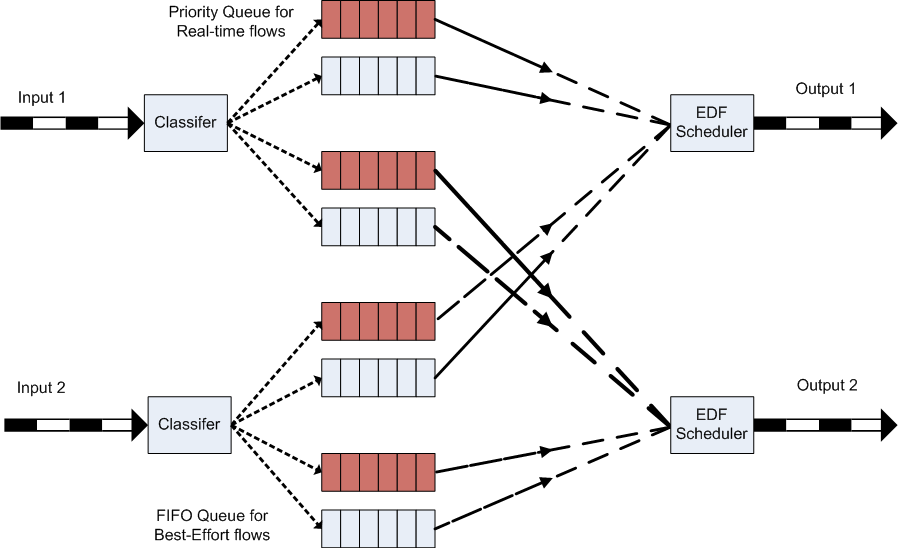
\includegraphics[width=8cm]{pics/Router.png}
\caption[Other Spec.]
{Structure of routers}\label{fig:RouterStructure}
\end{figure}

\subsection{Routing}
When a reservation path packet reaches a node and the calculated routing link 
to another router cannot afford the service time and transmission rate or delay 
bound for that reserving flow. The master node monitors all configurations of
real-time flows on the network so various routing policy can be employed to
achieve better performance, delay, power and so on.

The routing alogrithm is depth first search based on XY routing (try X
direction first). An example about routing is shown in Figure
\ref{fig:3FlowsEx} with three real-time flows.

\begin{itemize}
  \item Flow 1: PE7-> PE23
  \item Flow 2: PE6-> PE3
  \item Flow 3: PE5-> PE19
\end{itemize}

Flow 1 comes first and gets routed in blue path. Flow 2 comes later and gets
routed in read path.  When flow 2 gets routed through link from node 7 to node
8, the delay bound of flow 1 on that edge is modify, however, the total delay
bound of that flow still does not exceed the requested delay bound.

When flow 3 comes, it gets routed to node 7, however, it can not travel the
link from node 7 to 8 since the link utilization would exceed 1 if that link
has the third flow. The flow 3 then get routed to node 12 then reach the node.

\begin{figure}[htp]
\centering
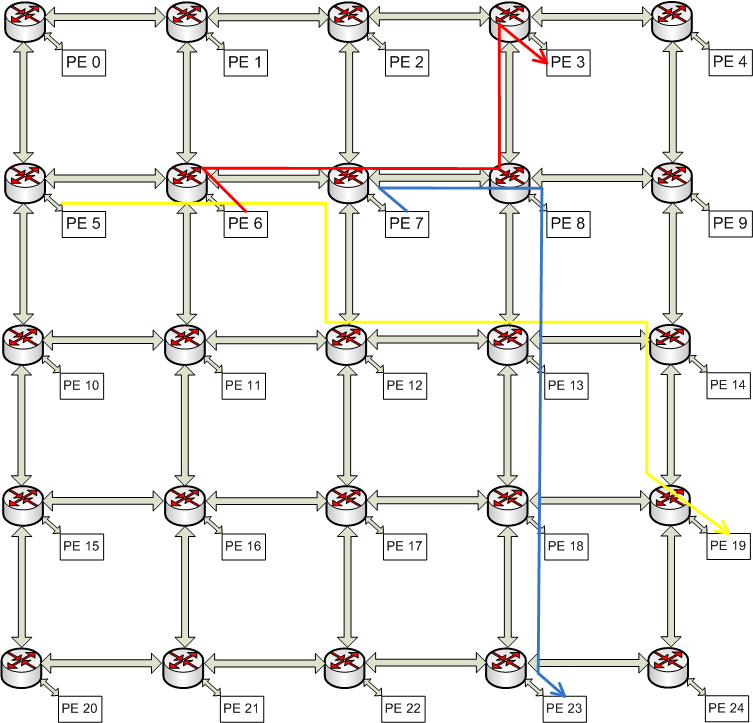
\includegraphics[width=8cm]{pics/Example.png}
\caption[Three flows example.]
{Example of three flows scheduled to share links}\label{fig:3FlowsEx}
\end{figure}

\section{Implementation}
Router micro-architecture can be implemented as in
\cite{Rexford98arouter},\cite{ZhangService} and extend \cite{PehDelayModel},
\cite{PehSpecPipeR} to have better performance.

Simulation program is written in SystemC based loosely on Noxim \cite{Noxim}.
To test our implementation, we initiate three real-time flows on the network as
in Figure \ref{fig:3FlowsEx}.

\begin{figure}[htp]
\centering
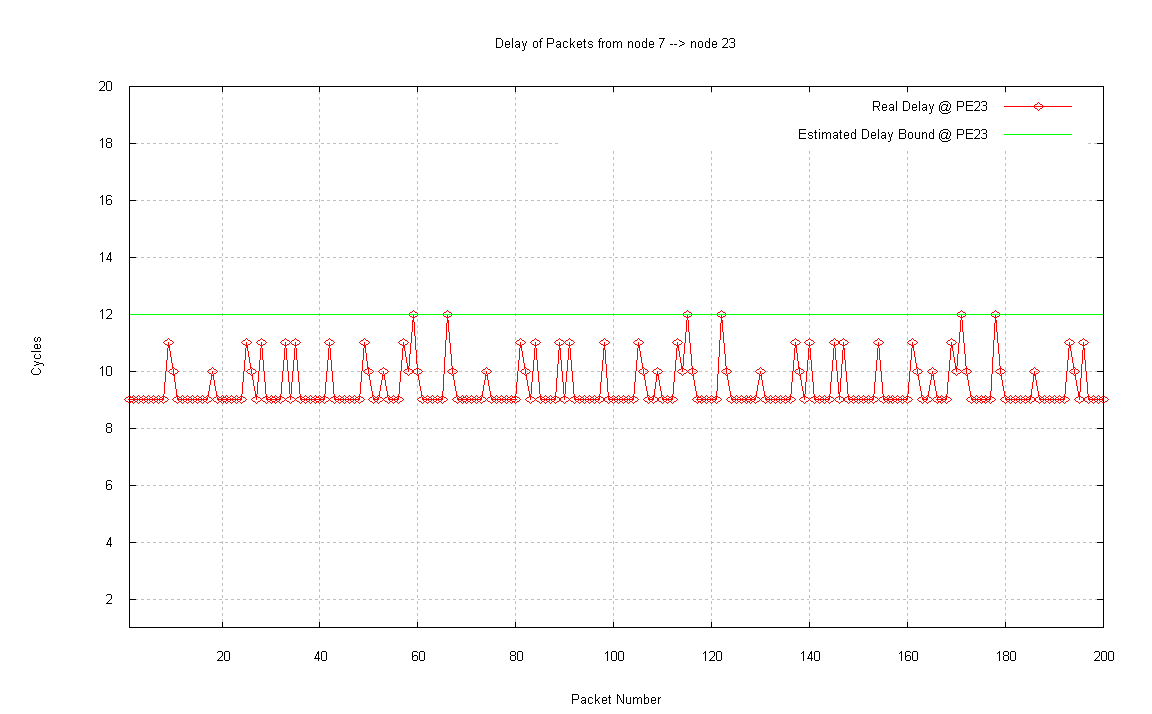
\includegraphics[width=8cm]{pics/PE23.png}
\caption[Flow from node 7 to node 23.]
{Real delay and estimated delay of real-time flow from node
7 to node 23}\label{fig:PE7PE23}
\end{figure}

\begin{figure}[htp]
\centering
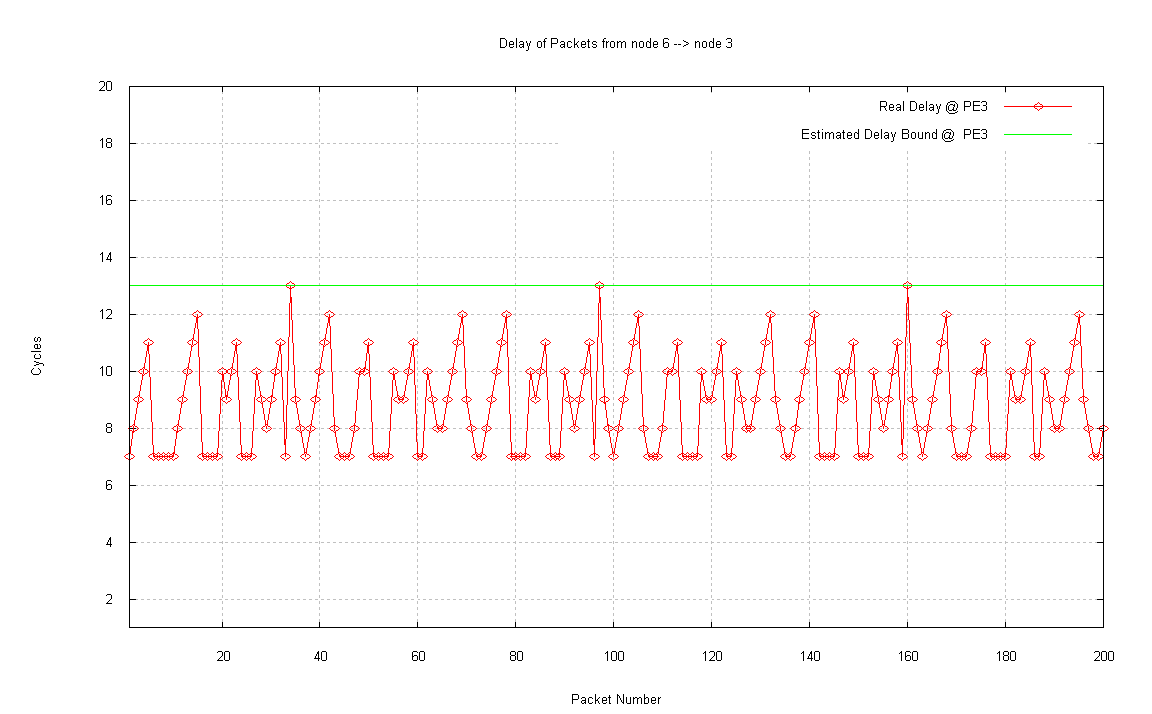
\includegraphics[width=8cm]{pics/PE3.png}
\caption[Three flows example.]
{Real delay and estimated delay of real-time flow from node
6 to node 3}\label{fig:PE6PE3}
\end{figure}

\begin{figure}[htp]
\centering
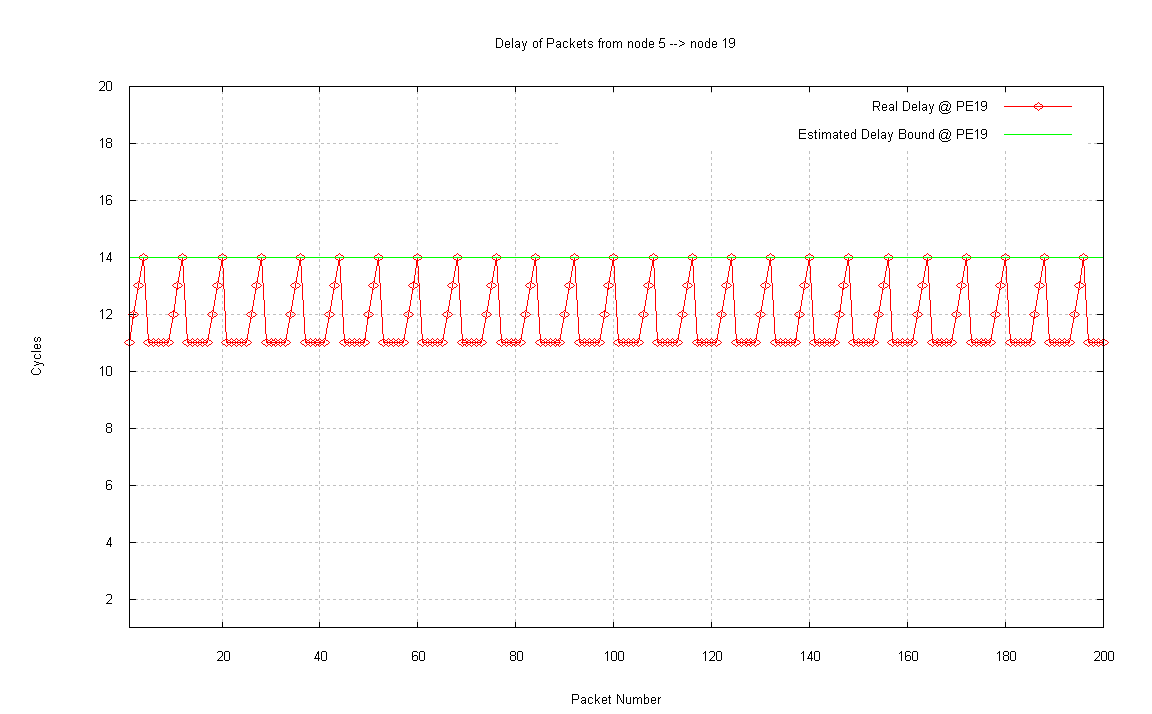
\includegraphics[width=8cm]{pics/PE19.png}
\caption[Three flows example.]
{Real delay and estimated delay of real-time flow from node
5 to node 19}\label{fig:PE5PE19}
\end{figure}

As we can see that the three flows interact with each other yet the delay of a
packet is never greater than the estimated delay bound. And the delay of these
flows is much more lower than the average delay in a best-effort network like
this (noxim original implementation), which is about more than {\em 5000}
cycles.

\bibliography{RTNoC}
\bibliographystyle{plain}

\end{document}.
